\section{System Overview}

In this research, a library called ``hils-connector'' is created. The purpose of
this library is to connect the ScenarioRunner and GRS program. The
``hils-connector'' is the interface that allows both programs to exchange data.
The library itself has two components: ``consumer'' (consumes sensor data, used
by GRS) and ``producer'' (produces sensor data by forwarding sensor data from
CARLA to consumer, used by ScenarioRunner).

The approach to use a library is chosen to reduce coupling between the library
and both main programs. The library can be loaded and linked optionally during
runtime and compile time to make better use of both computers' resources.

The communication protocol/method that is chosen for is ZeroMQ. ZeroMQ is chosen
because of its minimalism which could lead to improvement in communication
latency. Previously, ROS 2 was also considered, but ROS 2 has too many
abstraction layers and isn't supported by the OS version in AGX/RKB computer.
The AGX/RKB computer runs Ubuntu 18.04 which only supports up to ROS 1. Although
a bridge between ROS 2 and ROS 1, that bridge would only add overhead in the
communication process, therefore ROS was not chosen. Another communication
protocol that was considered is HTTP, which is used in the previous HILS system.
HTTP is also not chosen because of the additional overhead needed to parse
header and status code which is not needed in the HILS system. Thus, to maximize
the usage of computer resource and reduce possible overhead, ZeroMQ is chosen
over HTTP.

With this library approach, the system architecture can be seen in
Fig.~\ref{section-3-hils-deployment-diagram}. The two main programs,
ScenarioRunner and GRS, are connected to each other using hils-connector in a
local area network. Each library components are then connected using ZeroMQ.
CARLA is connected to the ScenarioRunner program using the CARLA Python API's
function calls.

\begin{figure}[htbp]
	\centerline{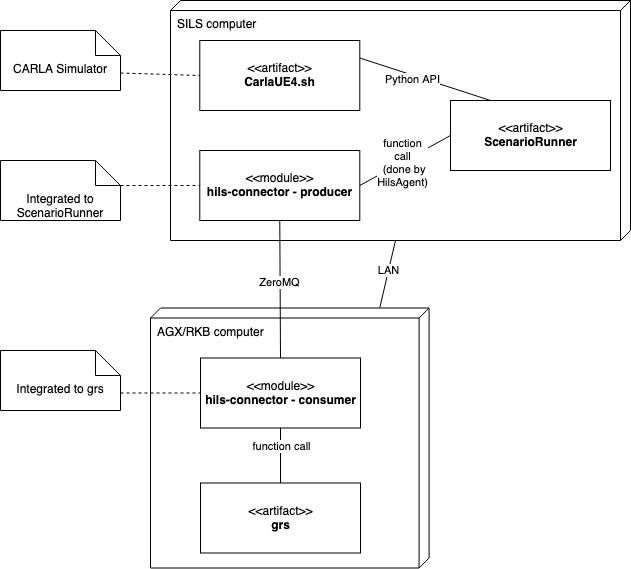
\includegraphics[width=0.4\textwidth]{resources/chapter-3/deployment-diagram-new-hils-EN.png}}
	\caption{HILS System Architecture}
	\label{section-3-hils-deployment-diagram}
\end{figure}

Then, as for how the system runs, it can be seen in
Fig.~\ref{section-3-hils-sequence-diagram}. Do note ScenarioRunner is called
``HILS agent'' in the diagram because HILS agent is the agent that is ran on
ScenarioRunner. To summarize how the system works:
\begin{enumerate}
	\item when CARLA steps, a sensor data is emitted,
	\item the producer component pushes it to the ZeroMQ socket,
	\item the consumer component waits for sensor data then pull from each
	      ZeroMQ socket,
	\item GRS will process that data to generate a control,
	\item the consumer component pushes the control to the ZeroMQ socket,
	\item the producer component will pull it and then send it to the
	      ScenarioRunner program, and
	\item ScenarioRunner will then apply the control to CARLA.
\end{enumerate}

\begin{figure}[htbp]
	\centerline{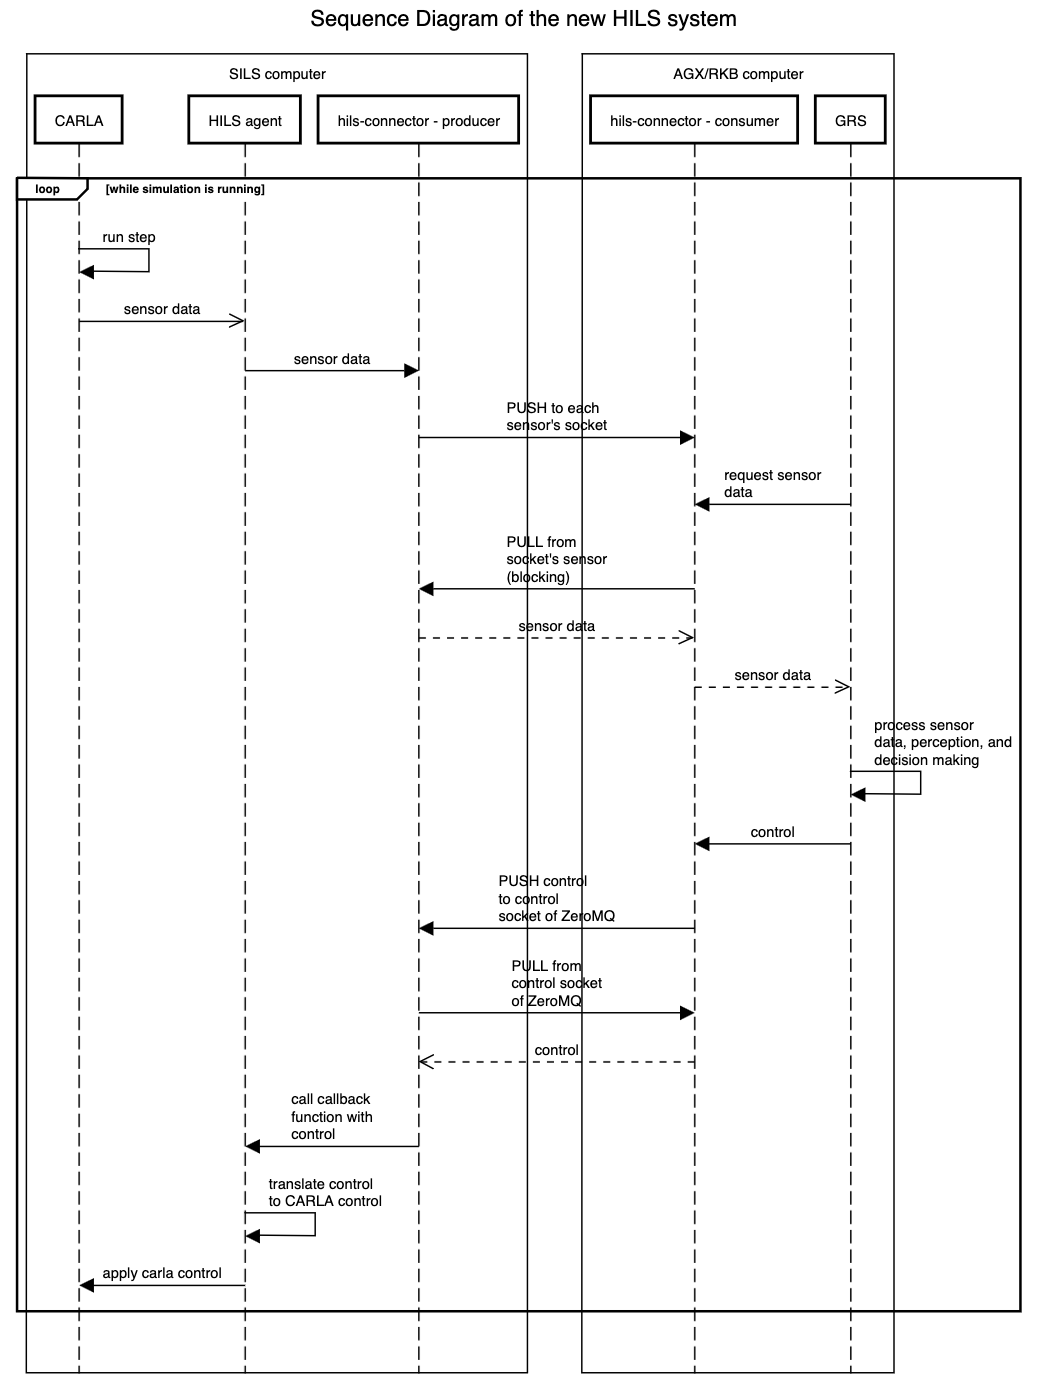
\includegraphics[width=0.5\textwidth]{resources/chapter-3/sequence-diagram-new-hils-kasar-EN.png}}
	\caption{HILS System Architecture}
	\label{section-3-hils-sequence-diagram}
\end{figure}

% \begin{table}[htbp]
% 	\caption{Table Type Styles}
% 	\label{tab1}
% 	\begin{center}
% 		\begin{tabular}{c c c c}
% 			\toprule
% 			\textbf{Table} & \multicolumn{3}{|c|}{\textbf{Table Column Head}}                                                         \\
% 			\cline{2-4}
% 			\textbf{Head}  & \textbf{\textit{Table column subhead}}           & \textbf{\textit{Subhead}} & \textbf{\textit{Subhead}} \\
% 			\midrule
% 			copy           & More table copy$^{\mathrm{a}}$                   &                           &                           \\
% 			\bottomrule
% 			\multicolumn{4}{l}{$^{\mathrm{a}}$Sample of a Table footnote.}
% 		\end{tabular}
% 	\end{center}
% \end{table}